%% =====================================================================
%%  Artifact Appendix for the paper
%%  "Snatcher: Apple Find My Network Exposes Your Lost Devices to Strangers"
%%  ACM CCS 2026 -- Artifact Evaluation
%%
%%  Conforms to the official CCS 2026 template (ccs2026-ae): same section
%%  structure (Abstract; Description & Requirements; Set Up; Evaluation
%%  Workflow with Major claims + Experiments).
%%  Build: pdflatex Snatcher_AE.tex  (run twice for cross-references).
%% =====================================================================
\documentclass[nonacm,sigconf]{acmart}

\usepackage{paralist}
\usepackage{listings}
\usepackage{xcolor}
\usepackage{subcaption}
\usepackage{dblfloatfix}   % fix placement/loss of full-width (figure*) floats
\usepackage{float}        % [H] to pin single-column figures next to their text

\settopmatter{printacmref=false}
\renewcommand\footnotetextcopyrightpermission[1]{}
\pagestyle{plain}

%% Allow several per-experiment figures to be placed (top/bottom/float pages)
%% without overflowing the float queue.
\setcounter{topnumber}{4}
\setcounter{bottomnumber}{4}
\setcounter{totalnumber}{8}
\renewcommand{\topfraction}{0.95}
\renewcommand{\bottomfraction}{0.95}
\renewcommand{\textfraction}{0.05}
\renewcommand{\floatpagefraction}{0.8}
%% Same, for full-width (figure*) floats -- several compete in this appendix.
\setcounter{dbltopnumber}{4}
\renewcommand{\dbltopfraction}{0.9}
\renewcommand{\dblfloatpagefraction}{0.7}
\setlength{\emergencystretch}{3em}

%% A lightweight style for shell / config snippets.
\definecolor{cmdbg}{gray}{0.96}
\lstdefinestyle{cmd}{
  basicstyle=\ttfamily\footnotesize,
  backgroundcolor=\color{cmdbg},
  breaklines=true,
  columns=fullflexible,
  keepspaces=true,
  frame=none,
  xleftmargin=0.5em,
  aboveskip=0.6em,
  belowskip=0.4em,
  literate={~}{{\textasciitilde}}1
}
%% Serial-log style: tighter, boxed, for the firmware console output.
\lstdefinestyle{log}{
  basicstyle=\ttfamily\scriptsize,
  backgroundcolor=\color{cmdbg},
  breaklines=true,
  columns=fullflexible,
  keepspaces=true,
  frame=single,
  framesep=3pt,
  rulecolor=\color{black!25},
  xleftmargin=0.2em,
  aboveskip=0.3em,
  belowskip=0.2em,
}
\lstset{style=cmd}

\begin{document}
%% All hyperlinks blue (set here so it wins over the class's hyperref setup).
\hypersetup{colorlinks=true,allcolors=blue}
\raggedbottom   % don't stretch sparse columns to a flush bottom (avoids mid-column gaps)
%% Compact float/caption spacing: pack figures tightly, no big gaps.
\setlength{\textfloatsep}{8pt plus 2pt minus 2pt}
\setlength{\floatsep}{8pt plus 2pt minus 2pt}
\setlength{\intextsep}{8pt plus 2pt minus 2pt}
\setlength{\abovecaptionskip}{4pt}
\setlength{\belowcaptionskip}{1pt}

\title{Snatcher: Apple Find My Network Exposes Your Lost Devices to Strangers}

%% Verify author order and the equal-contribution / corresponding-author notes.
\author{Zhenyu Ren}
\authornote{Zhenyu Ren and Yanbo Zhang contributed equally to this work.}
\email{zrenax@connect.ust.hk}
\affiliation{%
  \institution{The Hong Kong University of Science and Technology}
  \city{Hong Kong}
  \country{China}}
\author{Yanbo Zhang}
\authornotemark[1]
\email{yanbozhang@ust.hk}
\affiliation{%
  \institution{The Hong Kong University of Science and Technology}
  \city{Hong Kong}
  \country{China}}
\author{Boya Liu}
\email{bliuby@connect.ust.hk}
\affiliation{%
  \institution{The Hong Kong University of Science and Technology}
  \city{Hong Kong}
  \country{China}}
\author{Mo Li}
\authornote{Corresponding author.}
\email{lim@ust.hk}
\affiliation{%
  \institution{The Hong Kong University of Science and Technology}
  \city{Hong Kong}
  \country{China}}

\maketitle

\appendix
\section{Artifact Appendix}

\subsection{Abstract}
\textit{Snatcher} demonstrates that the mechanisms making Apple's Find My
network effective for owners also expose lost Apple devices to unauthorized
discovery, tracking, and physical theft by strangers. The attack relies solely
on a commodity Android smartphone and requires no specialized hardware. The
paper formalizes a progressive three-level attack: \textit{(Level~1)} Acoustic
direction finding; \textit{(Level~2)} Passive RSSI--IMU navigation; and
\textit{(Level~3)} De-anonymization via spatial--temporal clustering.

The released artifact includes the \texttt{SnatchAPP} Android application for
discovering and actuating nearby lost devices, two ESP32 firmware images as
evaluation targets, and representative raw data traces with offline analysis
code to verify the navigation attacks safely. The artifact is packaged as a Git
repository (also archived on Zenodo), is licensed under AGPL-3.0, and targets the
\emph{Artifacts Available}, \emph{Artifacts Evaluated (Functional and
Reusable)}, and \emph{Results Reproduced} badges.

\subsection{Description \& Requirements}
The repository is laid out as follows:

\noindent\begin{minipage}{\linewidth}
\begin{lstlisting}
Snatcher/
  SnatchAPP/                  # sound-play app (paper Table 1)
  esp32_airtag_mac_rotation/  # mimicked AirTag (paper Fig 11)
  esp32_sound_maker/          # sound trigger fw (paper Table 1)
  reproduce/                  # example traces + analysis (Python)
    1_timeout_disconnect_distance/  # lost-state (paper Fig 3)
    2_mac_rotation/           # MAC rotation (paper Table 2)
    3_acoustic_direction/     # Level 1 direction (paper Fig 6)
    4_rssi_navigation/        # Level 2 RSSI-IMU nav (paper Fig 8)
    5_clustering/             # Level 3 clustering (paper Fig 11)
    6_max_distance/           # attack range (paper Fig 14,15)
    7_navigation_traces/      # end-to-end traces (paper Fig 17)
  doc/                        # this artifact appendix
  README.md  LICENSE          # quick start + AGPL-3.0
\end{lstlisting}
\end{minipage}

\noindent The top-level \texttt{README} gives a quick start. \texttt{SnatchAPP}
and \texttt{esp32\_sound\_maker} actuate the non-owner sound trigger (paper
Table~1); \texttt{esp32\_airtag\_mac\_rotation} is the mimicked-AirTag target for
Level-3 clustering. The \texttt{reproduce/} folder holds seven self-contained
examples and is the primary, hardware-free verification path: each pairs a small
\texttt{data/} trace with Python scripts that print a result and write a figure,
reproducing one named result of the paper (named in the tree above and in each
experiment below). In total they reproduce the paper's \textbf{Figures~3, 6, 8,
11, 14, 15, and~17} and \textbf{Tables~1 and~2} --- the lost-state threat model,
the three attack levels, the maximum attack range, and the end-to-end navigation
cost.

\subsubsection{How to access}
\begin{compactitem}
  \item \textbf{Archived (permanent):} Zenodo concept DOI (resolves to the latest
        version), \url{https://doi.org/10.5281/zenodo.20693210}.
  \item \textbf{Development version:} \url{https://github.com/rzy0901/Snatcher}.
  \item \textbf{Anonymized mirror:} \url{https://anonymous.4open.science/r/Snatcher-4D25}.
\end{compactitem}

\subsubsection{Hardware dependencies}
\begin{compactitem}
  \item \textbf{Trace-based reproduction (E1--E7):} none --- any commodity PC
        with Python suffices.
  \item \textbf{Attacker device (E0):} one Android smartphone running
        Android~7.0 (API~24) or newer, with Bluetooth Low Energy, a stereo
        microphone (the \texttt{UNPROCESSED} audio source must be supported for
        Level~1), and a 9-axis IMU.
  \item \textbf{Evaluation targets (E0):} two ESP32-family boards
        (we used the ESP32-WROVER-Kit; ESP32-S3/C3 also work) --- one for the
        mimicked-AirTag firmware, one for the sound trigger. Optionally an
        AirTag/AirPods (Level~1) and an iPhone/Apple Watch (Level~2), \emph{owned
        by the evaluator, signed into an Apple~ID and placed in the Separated
        (Lost) state}, to validate against production hardware.
  \item USB cables to flash the ESP32 boards and to retrieve logs from the phone.
        No GPU is required.
\end{compactitem}

\subsubsection{Software dependencies}
\begin{compactitem}
  \item \textbf{Python} 3.8+ with \texttt{numpy}, \texttt{scipy},
        \texttt{pandas}, and \texttt{matplotlib} (\texttt{reproduce/requirements.txt}).
  \item \emph{Optional, to build the live components:} Android
        Studio\footnote{\url{https://developer.android.com/studio}}
        (Hedgehog~2023.1.1+, \texttt{compileSdk~34}, JDK~17, \texttt{adb}) and
        ESP-IDF\footnote{\url{https://github.com/espressif/esp-idf}}~v4.4+.
  \item The Android build pulls \texttt{MPAndroidChart} and AndroidX via Gradle;
        the ESP32 firmware derives from OpenHaystack (mimicked AirTag) and
        AirGuard (sound trigger).
\end{compactitem}

\subsubsection{Benchmarks}
All traces are self-collected with \texttt{SnatchAPP}, which logs synchronized
CSV streams---BLE scans (MAC, RSSI, payload, timestamp), IMU samples
(accelerometer/gyroscope/magnetometer, fused orientation, PDR position, step
count), and navigation RSSI (RSSI, phone heading, reconstructed position, target
heading)---plus raw stereo PCM audio with per-recording metadata. Each example
ships, in its \texttt{data/} folder, the processed trace it consumes, so the
analysis runs without collecting new measurements. The bulkier raw scan logs
behind these traces are retained locally (available on request), while
\texttt{1\_timeout\_disconnect\_distance/}, \texttt{2\_mac\_rotation/}, and
\texttt{6\_max\_distance/} also ship a representative raw capture under
\texttt{raw/} so the raw-to-trace derivation can be inspected. No personal or
third-party user data are included.

\subsubsection{Security, privacy, and ethical concerns}
\textit{Snatcher} is offensive --- it can discover, actuate, and physically
localize Apple Find My devices that are not the operator's. Evaluate it
\emph{only} against devices you own (commercial Apple devices you control, or the
provided ESP32 lab targets); never trigger sound on, connect to, or track a
third party's device. To avoid misuse, the released \texttt{SnatchAPP} omits the
on-device navigation- and clustering-assistance modules; the trace-based
reproduction still validates those algorithms offline from the shipped logs and
performs no live attack. Running it is otherwise safe: no destructive steps, no
privileged access, no security mechanisms disabled.

\subsection{Set Up}
A \emph{prebuilt} \texttt{SnatchAPP} APK (part~(A)) lets reviewers run the live
on-device attack (E0) in about a minute with no build --- \emph{we encourage
trying it}. \emph{Building} from source (parts~(A)/(B)) is optional, and the
trace-based reproduction (E1--E7) runs from the provided traces and Python code
(part~(C)) on any PC.

\subsubsection{Installation}
\noindent\textbf{(A) Android application.}
\emph{The fastest path is the prebuilt, signed APK --- no build needed:} download
\texttt{SnatchAPP.apk}\footnote{\url{https://github.com/rzy0901/Snatcher/raw/main/SnatchAPP/SnatchAPP.apk}}
and install it on any Android~7.0+ phone (open it on the device and allow
``install unknown apps'', or \texttt{adb install -r SnatchAPP.apk}). To build from
source instead, open \texttt{SnatchAPP/} in Android Studio (\emph{Run} installs
it), or:
\begin{lstlisting}
cd SnatchAPP
./gradlew assembleRelease
adb install -r app/build/outputs/apk/release/app-release.apk
\end{lstlisting}
On first launch, grant the requested permissions (Bluetooth scan/connect, fine
location, microphone, physical activity, and storage). Figure~\ref{fig:ae_install}
shows the partially-released app running from Android Studio.

\begin{figure}[tbp]
  \centering
  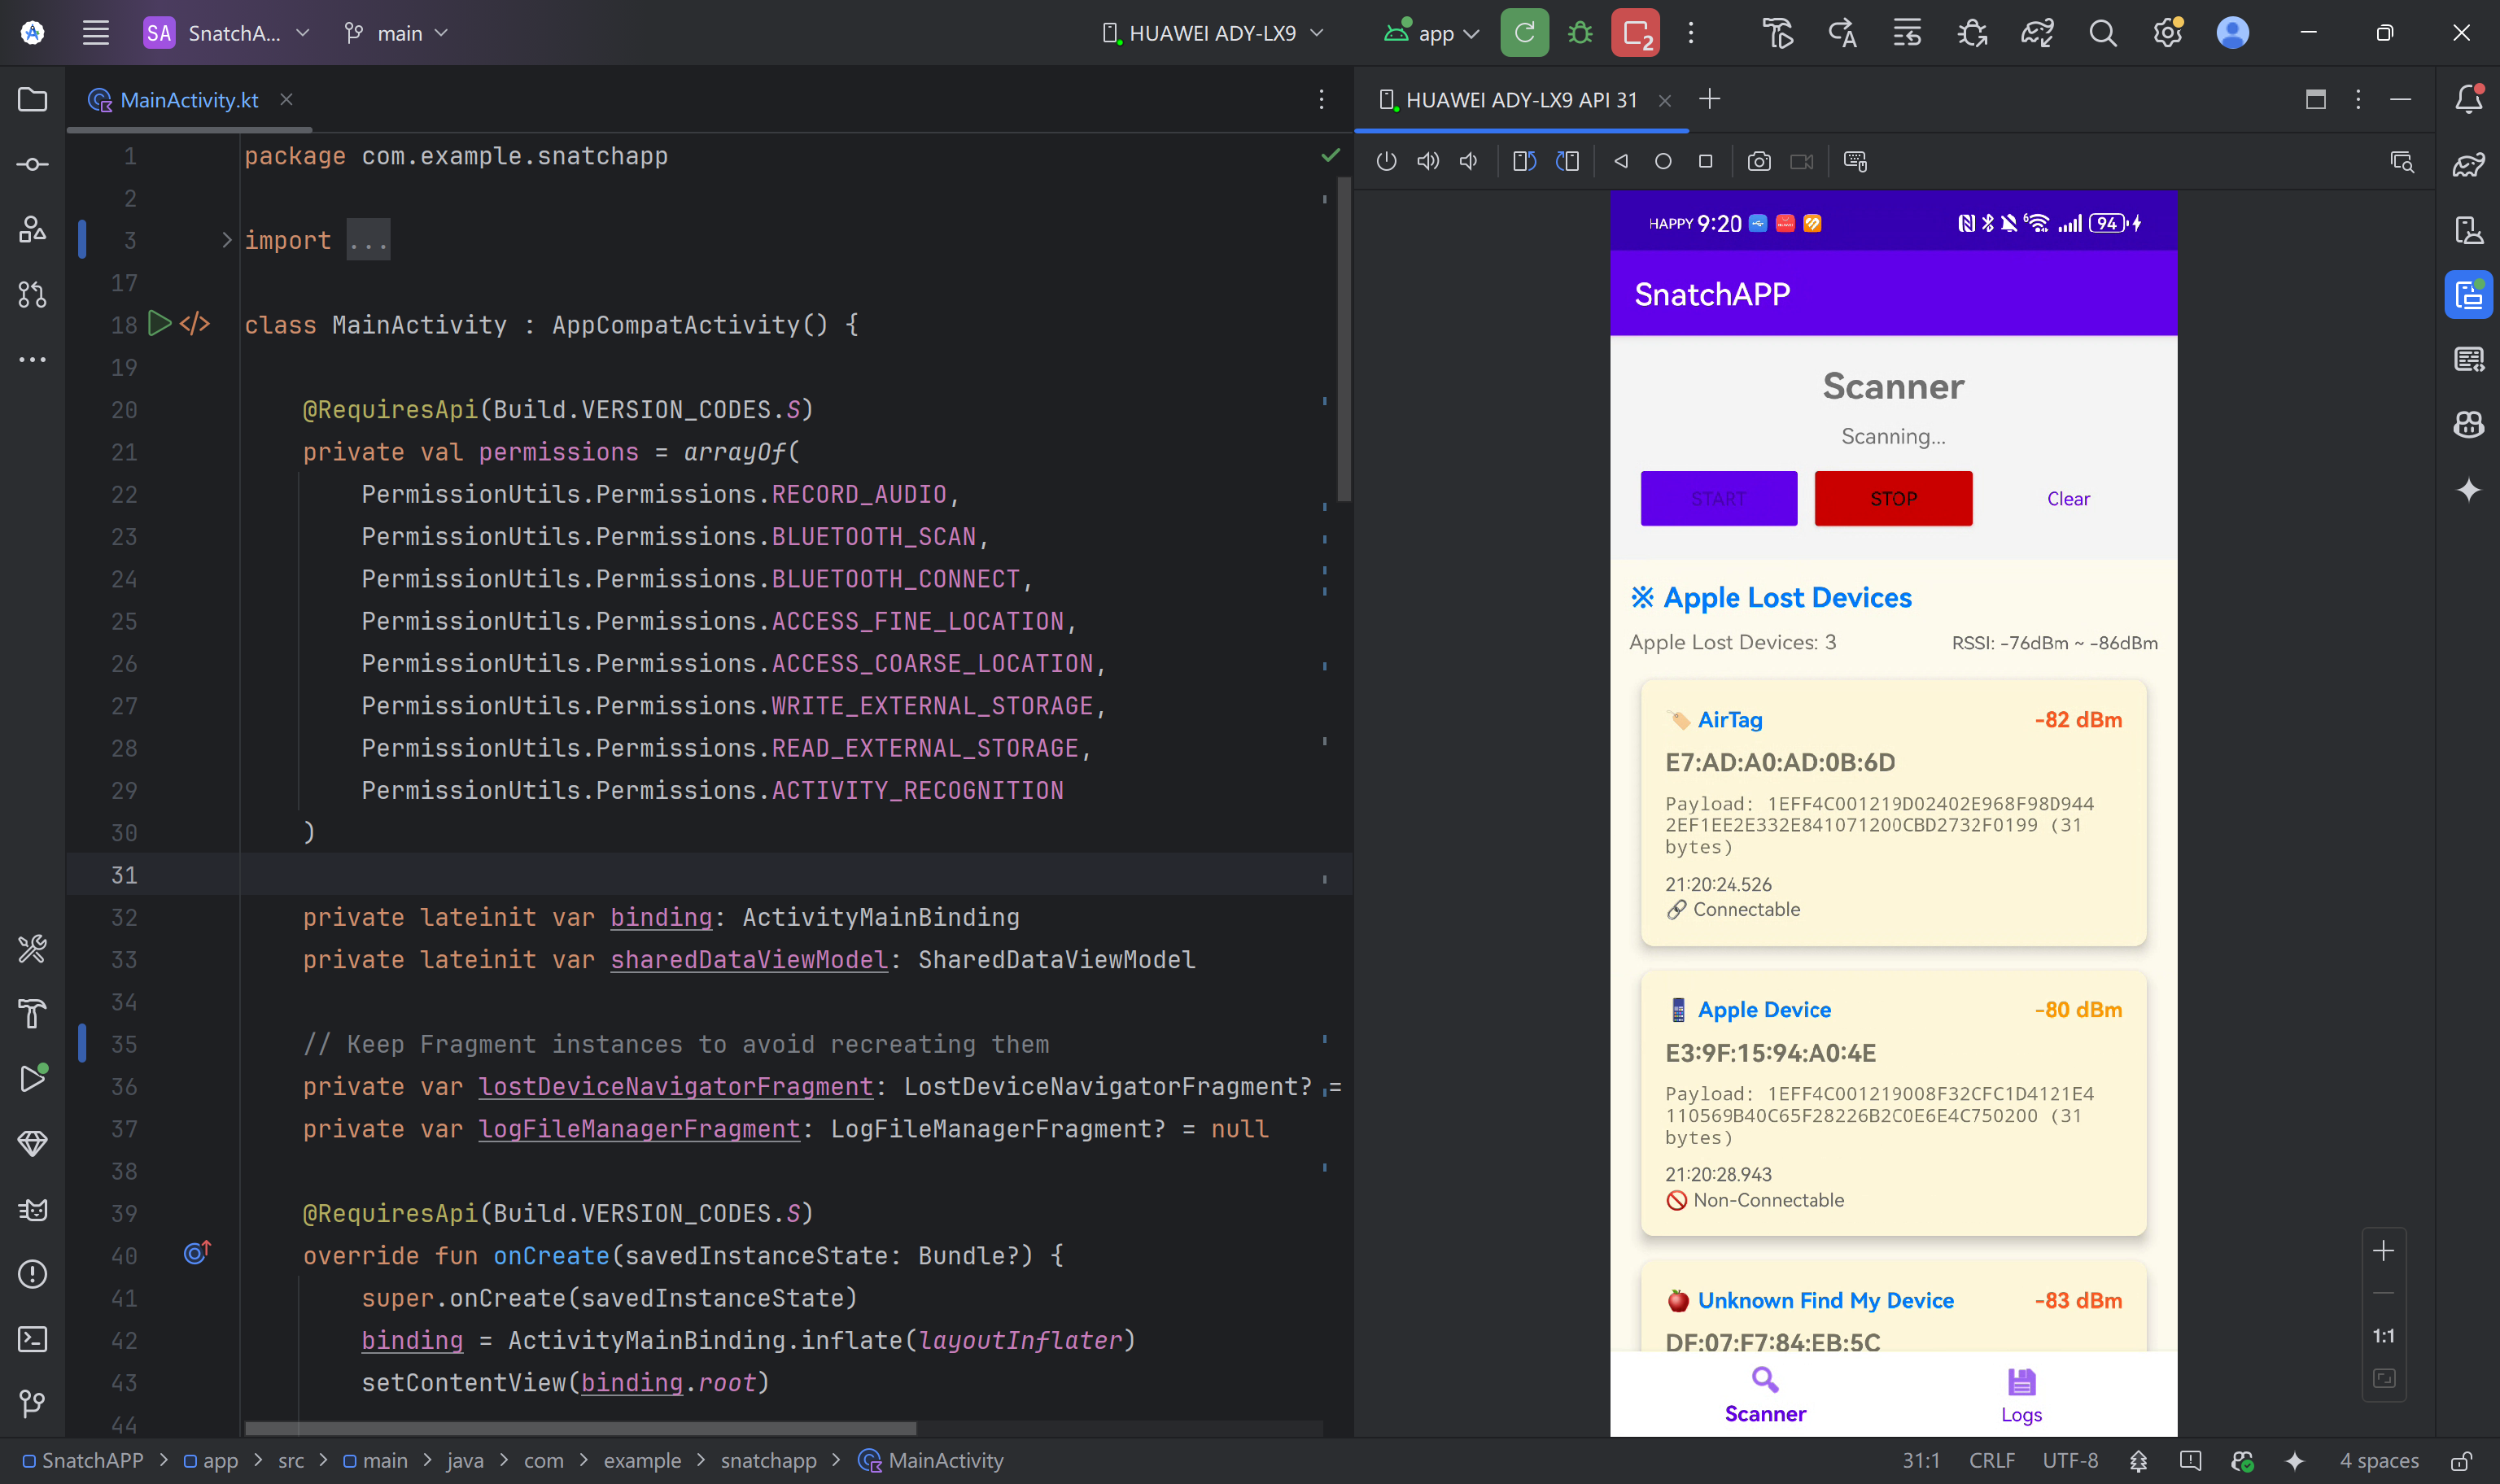
\includegraphics[width=0.88\linewidth]{figs/snatchapp_screenshot.png}
  \caption{The partially-released \texttt{SnatchAPP} built and run from Android
  Studio. The \textit{Scanner} screen lists nearby Apple lost devices with their
  type, MAC, RSSI, and Find My payload. Only lost-device discovery and the
  non-owner sound trigger are included; the navigation- and clustering-assistance
  modules are withheld to mitigate misuse.}
  \Description{Android Studio IDE on the left and a phone screen on the right running SnatchAPP, whose Scanner lists detected Apple lost devices with type, MAC, RSSI, and payload.}
  \label{fig:ae_install}
\end{figure}

\noindent\textbf{(B) ESP32 firmware (optional).}
For each firmware, source the ESP-IDF environment and, via
\texttt{idf.py menuconfig}, set the Bluetooth controller to \emph{BLE Only} and
enable Bluedroid. Then build, flash, and monitor:
\begin{lstlisting}
cd esp32_airtag_mac_rotation   # or esp32_sound_maker
idf.py set-target esp32
idf.py menuconfig              # set BLE Only + Bluedroid
idf.py -p <PORT> flash monitor
\end{lstlisting}
Before building, each firmware takes a one-line edit:
\begin{compactitem}
  \item \emph{Mimicked AirTag} (\texttt{openhaystack\_main.c}): set
        \texttt{DEVICE\_ID} (labels co-located devices) and the MAC-rotation
        period (paper: 10--60\,s).
  \item \emph{Sound trigger} (\texttt{main.c}): set \texttt{device\_type} and
        \texttt{target\_mac} to the victim accessory (read its MAC with
        \texttt{SnatchAPP} or nRF~Connect\footnote{\url{https://www.nordicsemi.com/Products/Development-tools/nRF-Connect-for-mobile}}).
\end{compactitem}
The serial monitor confirms each firmware runs (Figure~\ref{fig:ae_fw}): the
mimicked AirTag shuffles its MAC on schedule, and the sound trigger plays a
non-owner sound on a real Apple accessory (AirTag or AirPods; paper Table~1).

\begin{figure}[t]
\begin{lstlisting}[style=log]
--- (a) Mimicked AirTag: DEVICE_ID + 30 s MAC rotation ---
open_haystack: Device ID (ground truth): 0x01
open_haystack: MAC shuffle period: 30 seconds
open_haystack: using device address: fc ff ff ff 13 00
open_haystack: MAC shuffle timer started (period: 30 s)
open_haystack: Generated random MAC: dc 73 62 6a 46 db
open_haystack: MAC address shuffled, adv. restarts
open_haystack: Generated random MAC: dc 20 3c ac 11 bf
open_haystack: MAC address shuffled, adv. restarts
--- (b) Sound trigger: non-owner sound on a real AirTag ---
Connected, start service discovery...
AirTag service found: start=0x005D end=0xFFFF
Characteristic found, handle=0x005F. Sending sound play
AirTag: Sent sound play command (value=0xAF)
AirTag: Sound playback command sent successfully
\end{lstlisting}
  \caption{ESP32 firmware serial logs. (a)~the mimicked-AirTag firmware
  advertises under a ground-truth \texttt{DEVICE\_ID} and rotates its MAC every
  30\,s; (b)~the sound-maker firmware connects to a real AirTag and sends the
  non-owner sound-play command (paper Table~1). Full screenshots:
  \href{https://github.com/rzy0901/Snatcher/blob/main/doc/figs/fw_mac_rotation.png}{\texttt{doc/figs/fw\_mac\_rotation.png}},
  \href{https://github.com/rzy0901/Snatcher/blob/main/doc/figs/fw_soundplay.png}{\texttt{fw\_soundplay.png}}.}
  \Description{ESP32 serial logs rendered as text. (a) the mimicked-AirTag firmware prints its Device ID, MAC shuffle period, and successive random MAC addresses. (b) the sound-maker firmware connects to an AirTag, finds the Find My service, and reports the sound-play command was sent successfully.}
  \label{fig:ae_fw}
\end{figure}

\noindent\textbf{(C) Reproduction environment.}
\begin{lstlisting}
cd reproduce
python -m venv .venv && source .venv/bin/activate
pip install -r requirements.txt
\end{lstlisting}

\subsubsection{Basic test}
After installing the reproduction environment, run the acoustic example as a
quick functionality check:
\begin{lstlisting}
cd reproduce/3_acoustic_direction && python acoustic_example.py
\end{lstlisting}
It prints the detected arrival level ($\approx-42.8$\,dB), confirming the
toolchain is installed. With the prebuilt APK, E0 below is the live demo.

\subsection{Evaluation Workflow}
The evaluation is one functional check (E0) and seven reproduction experiments
(E1--E7), which run from the provided data with no Apple hardware; the
recommended E0 demo needs only an Android phone with the prebuilt APK. The
aggregate field results (per-level success rates, paper Figure~16, and averaged
end-to-end navigation times) need extensive real-world trials and are out of
automated scope; the artifact provides the implementation and logging to repeat
them.

\subsubsection{Major claims}
\begin{compactitem}
\item[(C1):] A separated device becomes discoverable quickly and at area scale:
  it enters its advertising lost state within minutes of the owner leaving, and
  the owner's BLE link drops at $\sim$10--20\,m across diverse indoor scenes
  (paper Figure~3). Validated by (E1).
\item[(C2):] Find My MAC-address rotation is slow enough to track: Apple
  \emph{accessories} keep one address for $\sim$24\,h, versus a fixed
  $\sim$15\,min (iPhone) or $\sim$19--36\,min (Apple~Watch) ---
  Vulnerability~III, paper Table~2. Validated by (E2).
\item[(C3):] A non-owner can find the \emph{direction} to a lost accessory that
  supports non-owner sound play (e.g.,\ AirTag, AirPods) by triggering its sound
  and comparing per-orientation loudness (Level~1, paper Figure~6). Validated by (E3).
\item[(C4):] A \emph{silent} lost device can be navigated to by fusing its BLE
  RSSI with phone IMU/PDR (Level~2, paper Figure~8). Validated by (E4).
\item[(C5):] The rotating MAC addresses of co-located lost devices can be
  re-associated into per-device clusters, defeating MAC-address randomization
  (Level~3, paper Figure~11). Validated by (E5).
\item[(C6):] The attack operates at practical range: a lost device stays
  BLE-discoverable out to tens of metres, and the non-owner sound trigger is
  effective at close range, both degrading gracefully with distance (paper
  Figures~14--15). Validated by (E6).
\item[(C7):] Under all three levels the attacker's reconstructed walking
  trajectory converges on the target, as sampled from the end-to-end navigation
  evaluation (paper Figure~17). Validated by (E7).
\end{compactitem}

\subsubsection{Experiments}

\noindent\textbf{(E0) Live on-device demo of the attack primitives}
[\emph{strongly recommended}; $\sim$10~person-min; just install the APK].
Install the prebuilt \texttt{SnatchAPP} APK (part~(A)), open the
\textit{Scanner}, and watch it discover the \emph{real} Apple devices in the
Separated (Lost) state broadcasting around you (usually several in any public
space). Then,
against a target you control (an AirTag/AirPods you own placed in Lost mode, or
the provided ESP32 mimicked-AirTag), confirm each primitive operates end to end:
\begin{compactenum}
  \item \textbf{Cleartext discovery (Vuln.~I).} On the \textit{Scanner}, verify
        each lost device is detected and identified from its Find My advertisement
        (the app filters the \texttt{FF\,4C\,00\,12\,19} prefix and decodes the
        device-type byte, e.g.\ AirTag, AirPods).
  \item \textbf{Unauthenticated actuation (Vuln.~II).} Tap a connectable lost
        device, open its detail view, and choose \emph{Play Sound \& Record}: with
        no pairing or authentication, the app records stereo audio, connects, and
        plays the non-owner alert sound (Figure~\ref{fig:ae_soundplay}; confirm it
        sounds on a real AirTag/AirPods or the sound-trigger ESP32). The recording
        (\texttt{audio\_left/right\_*.pcm} $+$ a \texttt{*\_metadata} file) is the
        Level-1 acoustic input for E3 (top mic = right channel).
  \item \textbf{Passive RSSI/IMU logging (Vuln.~III).} On the data-collection
        screen, confirm the app records the lost device's RSSI together with the
        phone's IMU motion, producing the synchronized logs that E4/E5 consume.
\end{compactenum}

\begin{figure}[tbp]
  \centering
  \begin{subfigure}[t]{0.28\linewidth}
    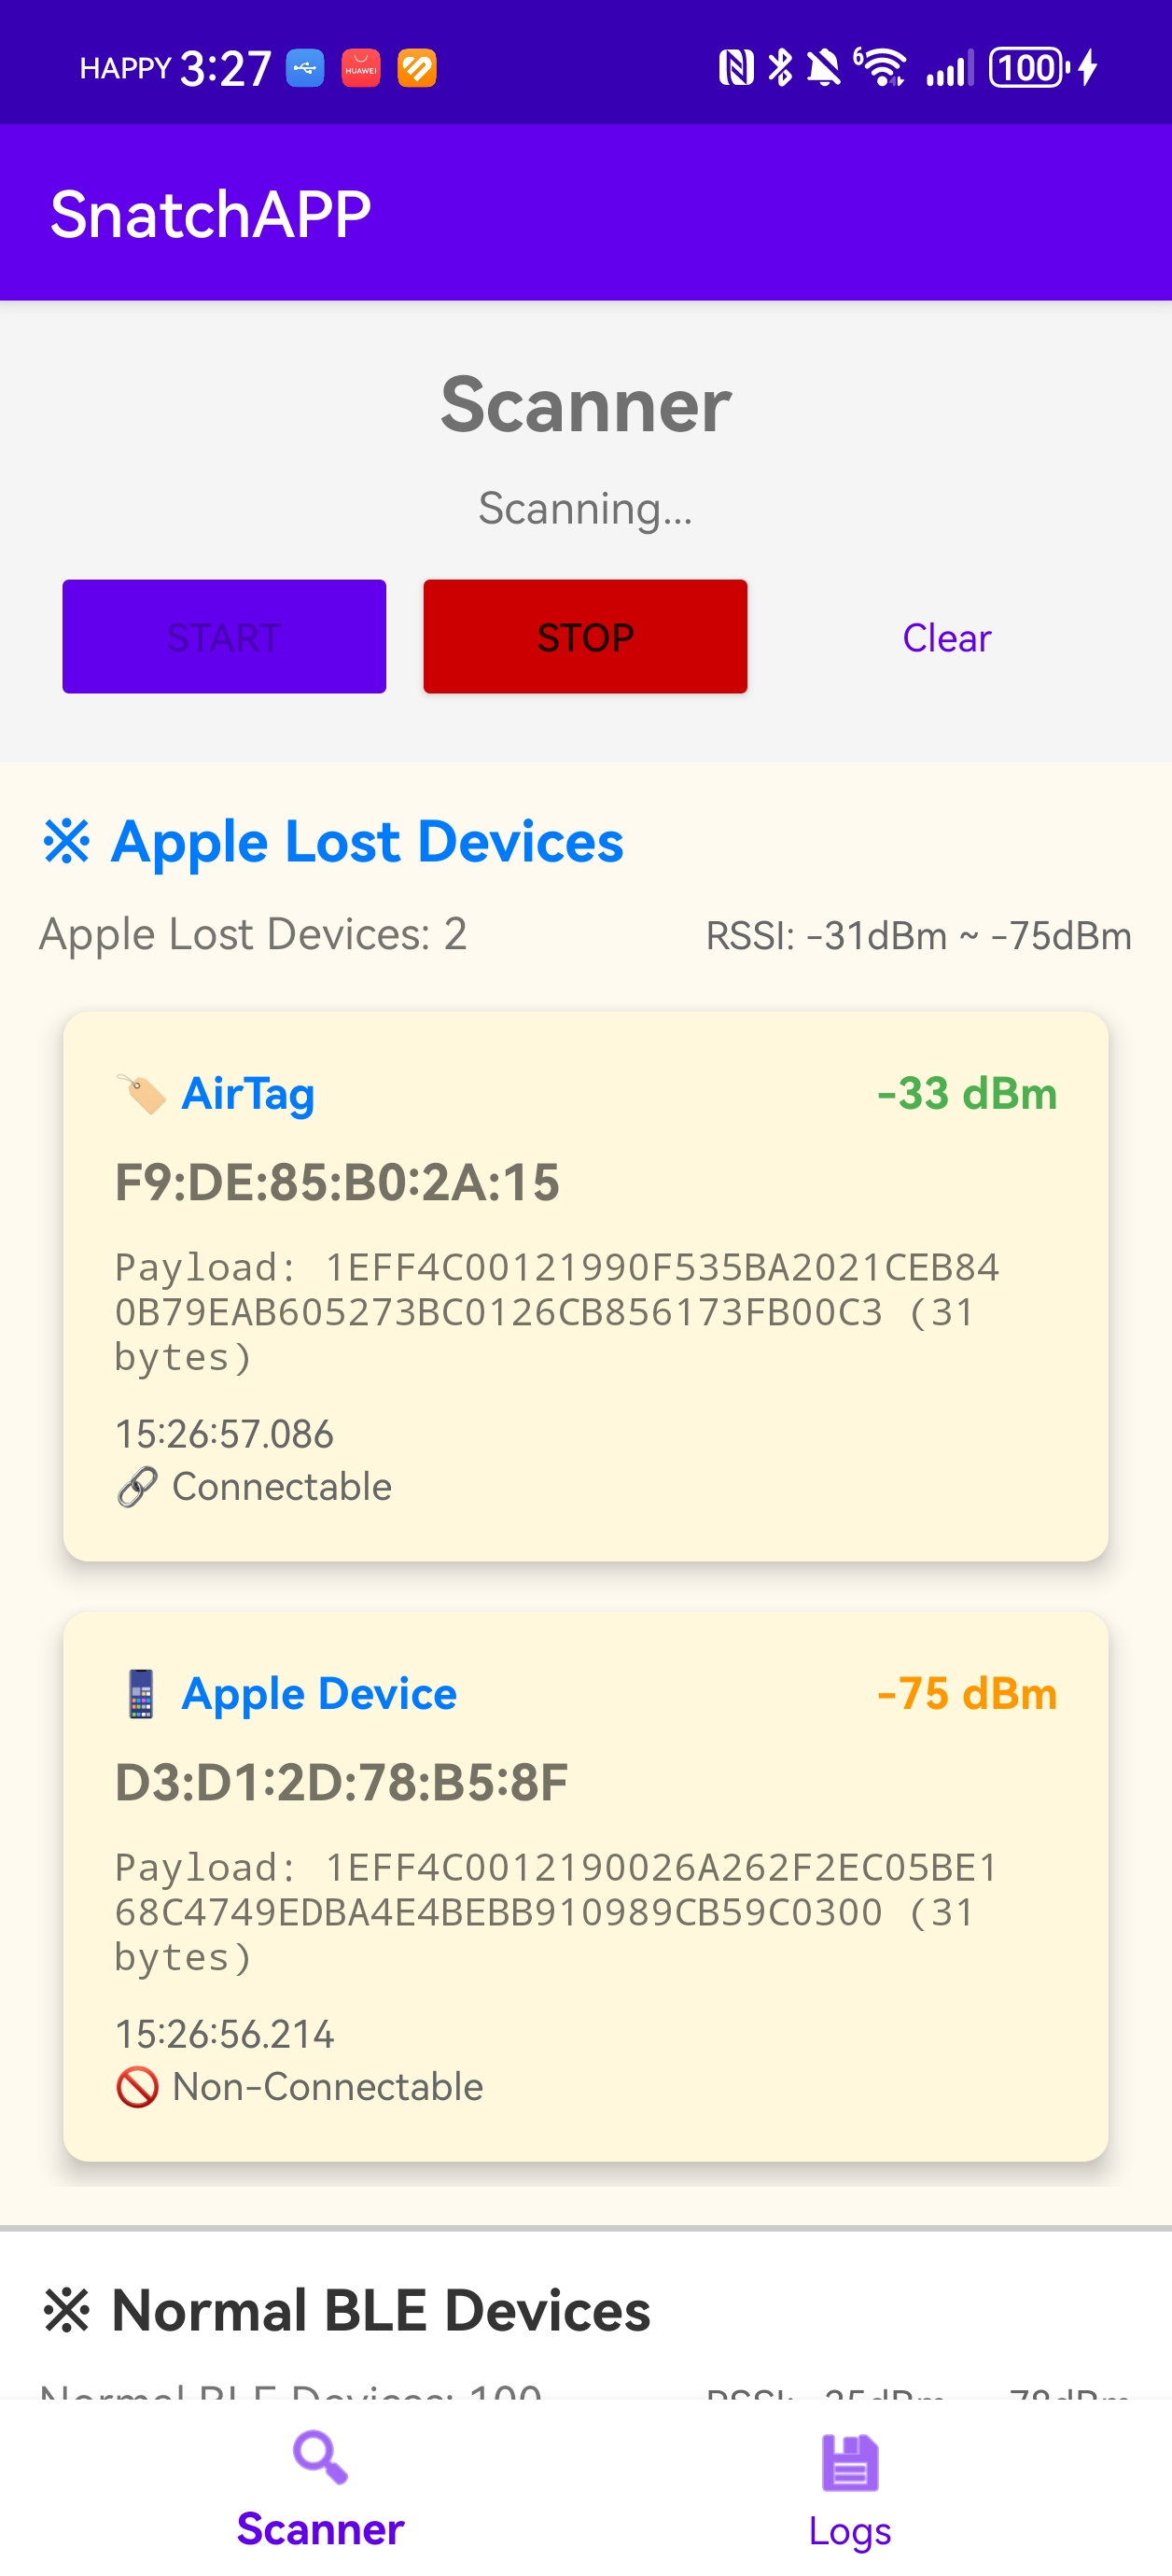
\includegraphics[width=\linewidth]{figs/soundplay_scan.jpg}
    \caption{\textit{Scanner}: tap a connectable lost device.}
    \label{sf:sp_scan}
  \end{subfigure}\hfill
  \begin{subfigure}[t]{0.28\linewidth}
    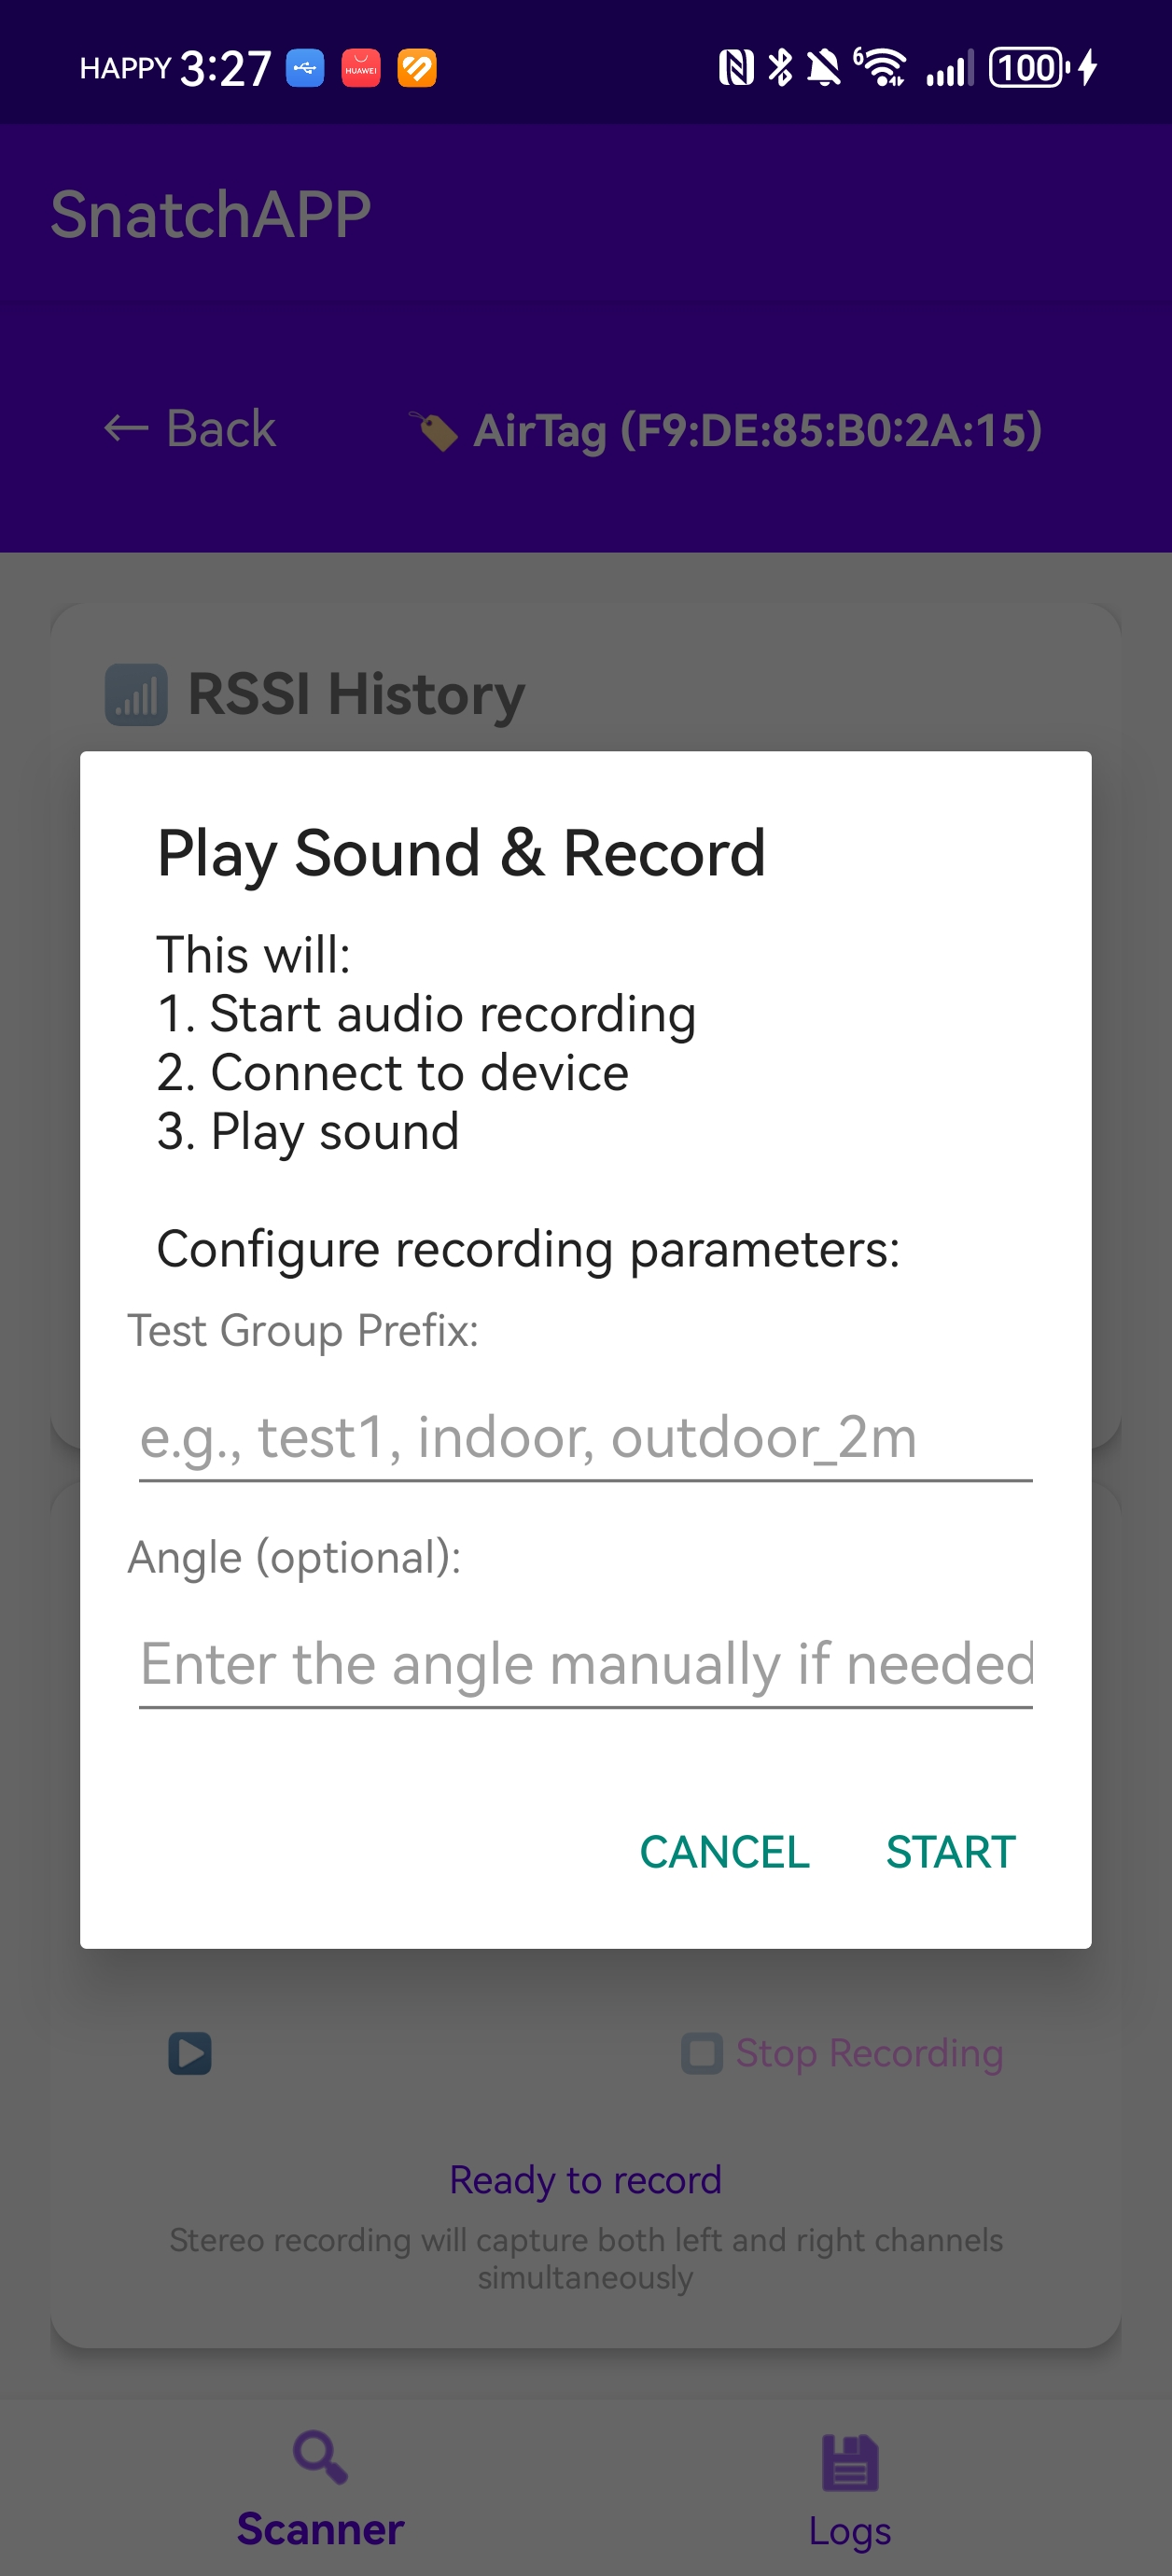
\includegraphics[width=\linewidth]{figs/soundplay_dialog.jpg}
    \caption{\emph{Play Sound \& Record}: record, connect, play.}
    \label{sf:sp_dialog}
  \end{subfigure}\hfill
  \begin{subfigure}[t]{0.28\linewidth}
    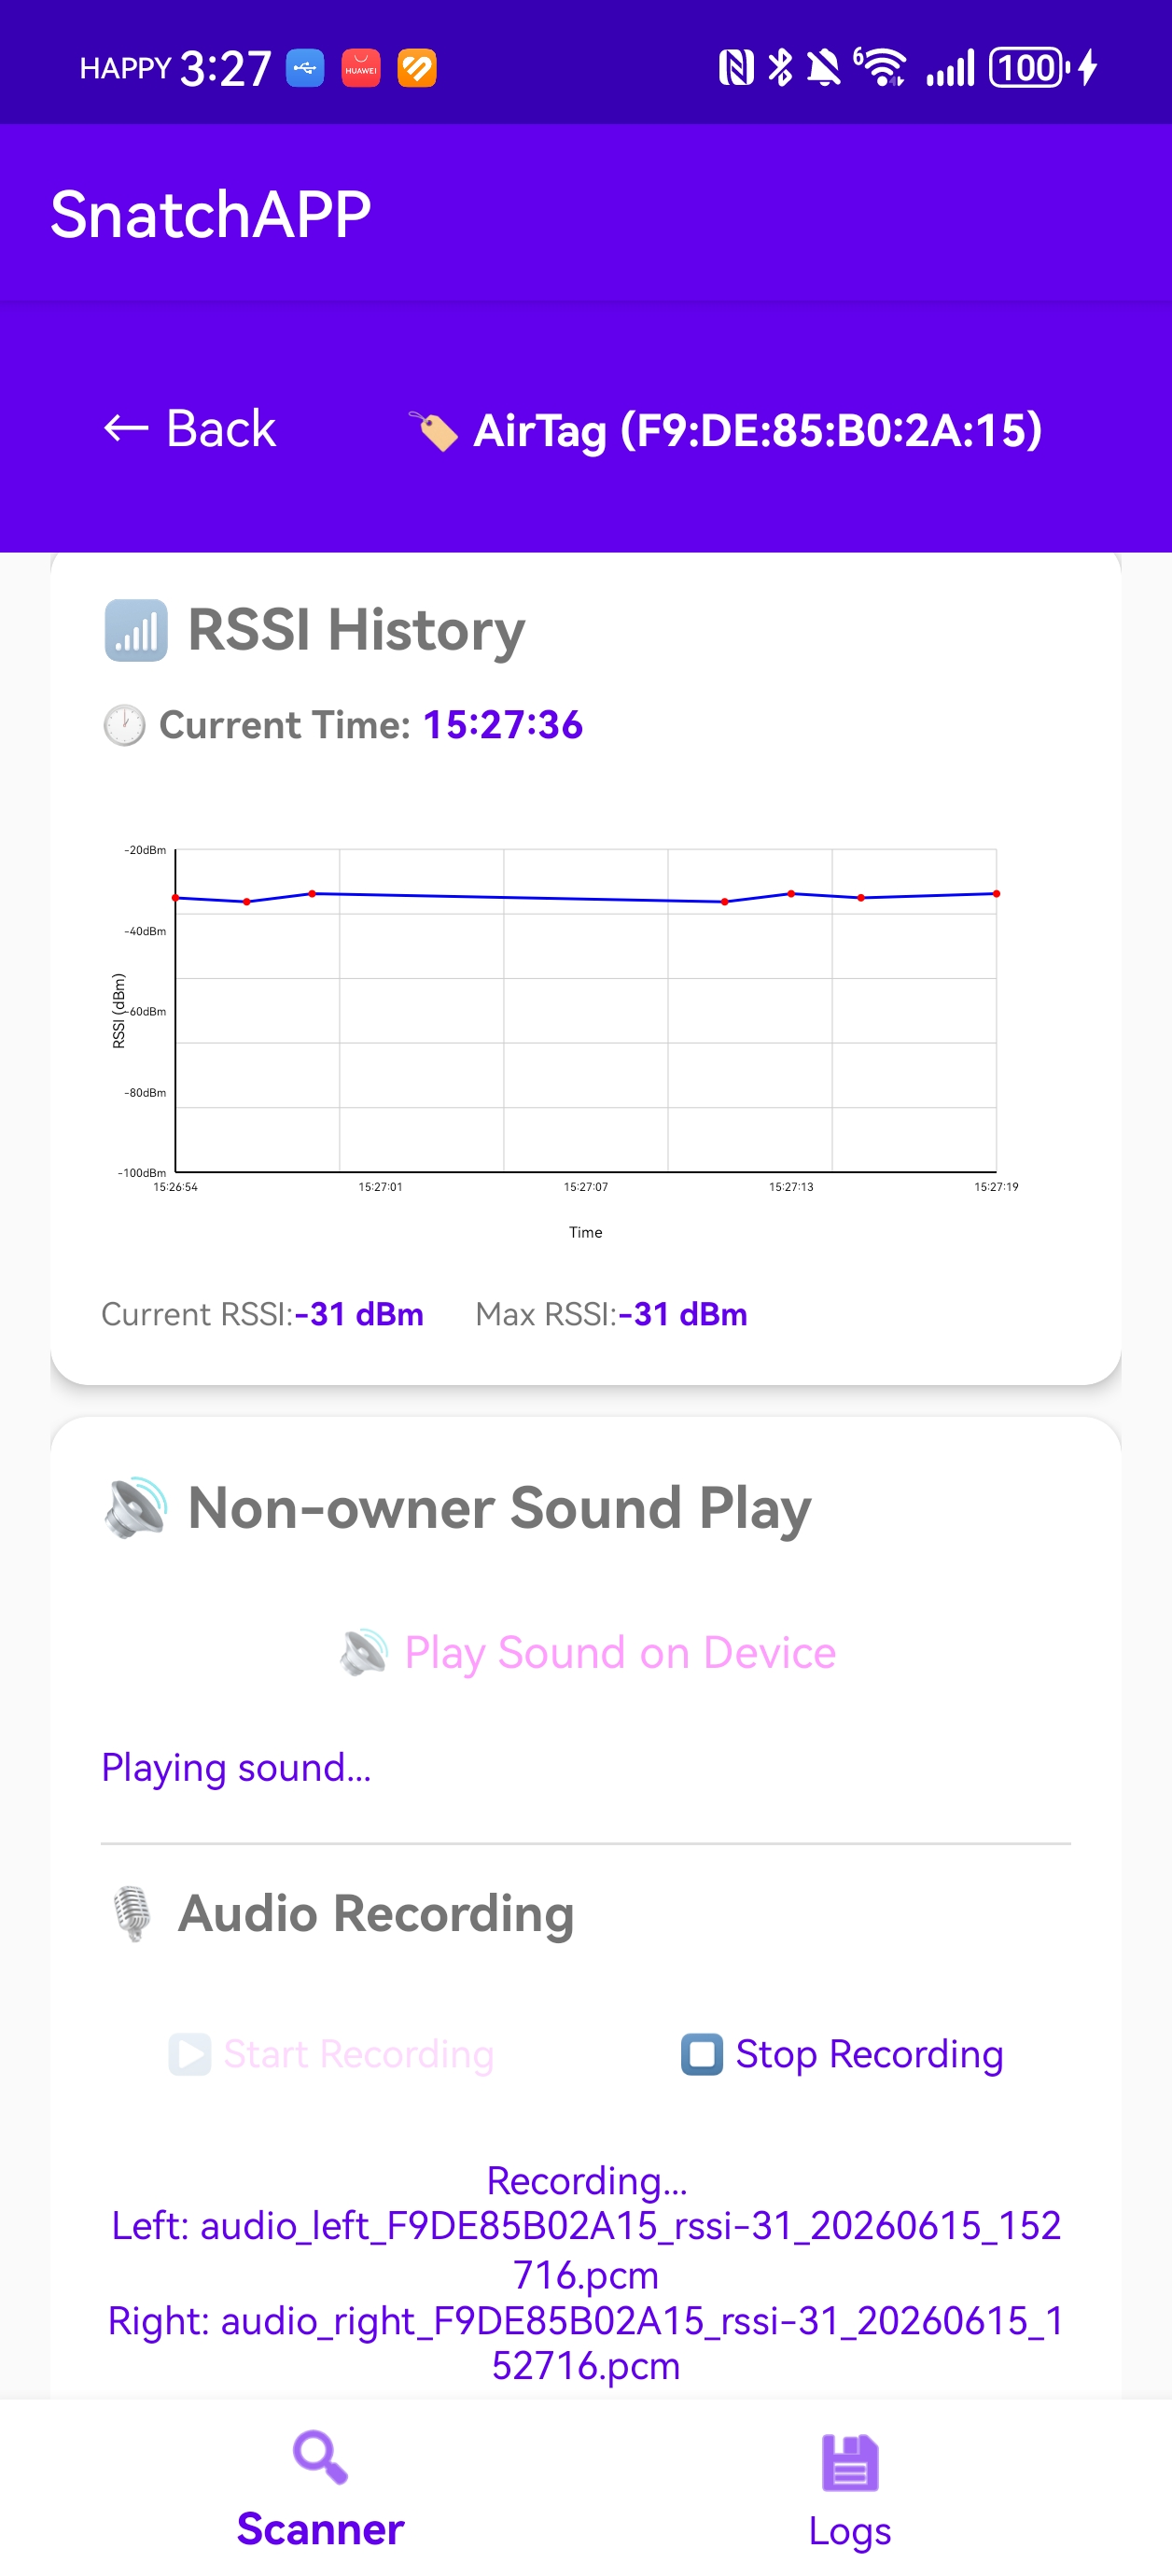
\includegraphics[width=\linewidth]{figs/soundplay_play.jpg}
    \caption{The alert plays; stereo audio is recorded.}
    \label{sf:sp_play}
  \end{subfigure}
  \caption{E0, non-owner sound trigger (Vuln.~II). On the \textit{Scanner} a
  connectable lost device is tapped (a); \emph{Play Sound \& Record} (b) starts a
  stereo recording, connects with no authentication, and plays the alert (c),
  saving \texttt{audio\_left/right\_*.pcm}.}
  \Description{Three phone screenshots: the SnatchAPP scanner listing Apple lost devices; a Play Sound and Record dialog listing the steps start-recording, connect, play; and the device detail screen showing "Playing sound" and an active stereo audio recording with the left/right PCM filenames.}
  \label{fig:ae_soundplay}
\end{figure}

Expected: the device is discovered, the alert plays, and the session writes its
outputs under the app's external files directory --- the BLE/IMU logs
(\texttt{ble\_scan\_*.csv}, \texttt{imu\_data\_*.csv}, \texttt{lost\_device\_*.csv},
\texttt{NavRSSI\_*.csv}) under \texttt{Documents/SnatchAPP\_Logs}, and the sound recordings
(\texttt{audio\_left/right\_*.pcm}) under \texttt{Music} --- demonstrating the
artifact is \emph{Functional}. Copy them off most simply by connecting the
phone over USB and opening either folder in a file browser
(Figure~\ref{fig:ae_logs}), or via ADB:
\begin{lstlisting}
adb pull /sdcard/Android/data/com.example.snatchapp/files/Documents/SnatchAPP_Logs
adb pull /sdcard/Android/data/com.example.snatchapp/files/Music
\end{lstlisting}

\begin{figure}[tbp]
  \centering
  \begin{subfigure}[b]{0.78\linewidth}
    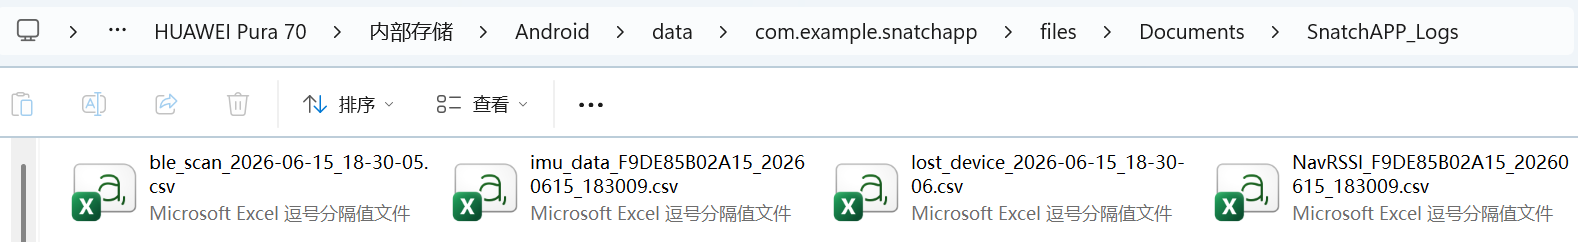
\includegraphics[width=\linewidth]{figs/filebrowser_logs.png}
    \caption{The BLE/IMU scan-log folder.}
    \label{sf:fb_logs}
  \end{subfigure}
  \\[5pt]
  \begin{subfigure}[b]{0.78\linewidth}
    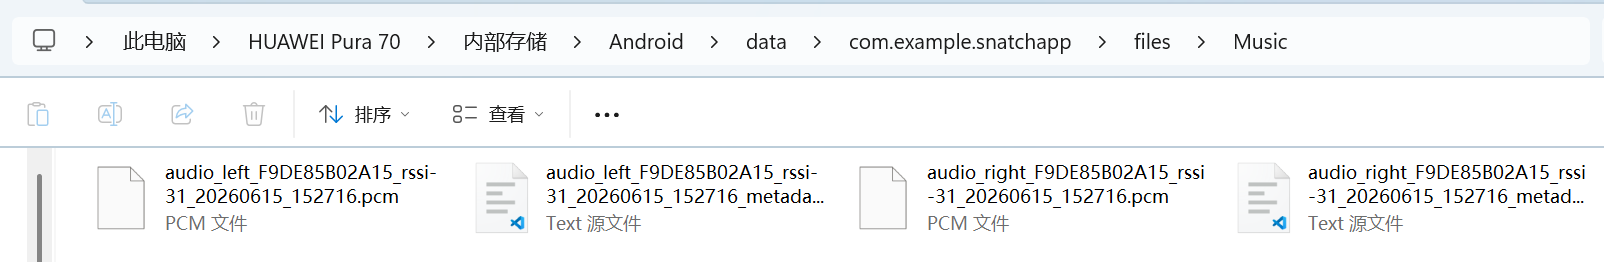
\includegraphics[width=\linewidth]{figs/filebrowser_audio.png}
    \caption{The triggered-sound recording folder.}
    \label{sf:fb_audio}
  \end{subfigure}
  \caption{E0 output retrieval without ADB: with the phone connected over USB,
  both the scan logs (a) and the triggered-sound recordings (b) are visible
  directly in a file browser and can be copied off.}
  \Description{Two file-browser windows: one showing the Documents/SnatchAPP_Logs folder with ble_scan, imu_data, lost_device and NavRSSI CSV files; the other showing the Music folder with audio_left/right PCM files and metadata.}
  \label{fig:ae_logs}
\end{figure}

\noindent\textbf{(E1) Lost-state onset (paper Figure~3)} [5~person-min]. How quickly,
and from how far, a separated device starts advertising in its lost state ---
the precondition for discovery.
\noindent\textbf{Preparation:} \texttt{cd reproduce/1\_timeout\_disconnect\_distance}.\\
\textbf{Execution:} \texttt{python plot.py}.\\
\noindent\textbf{Results:} a two-panel figure (Figure~\ref{fig:ae_onset}).
\emph{(a)}~the lost-state timeout per device on a log axis --- AirTag
$\sim$12\,min, AirPods longer but variable, Apple~Watch $\sim$13\,s;
\emph{(b)}~the owner-to-device disconnect distance stays at $\sim$10--20\,m
across four indoor scenes. These reproduce Figure~3 of the paper.

\begin{figure}[H]
  \centering
  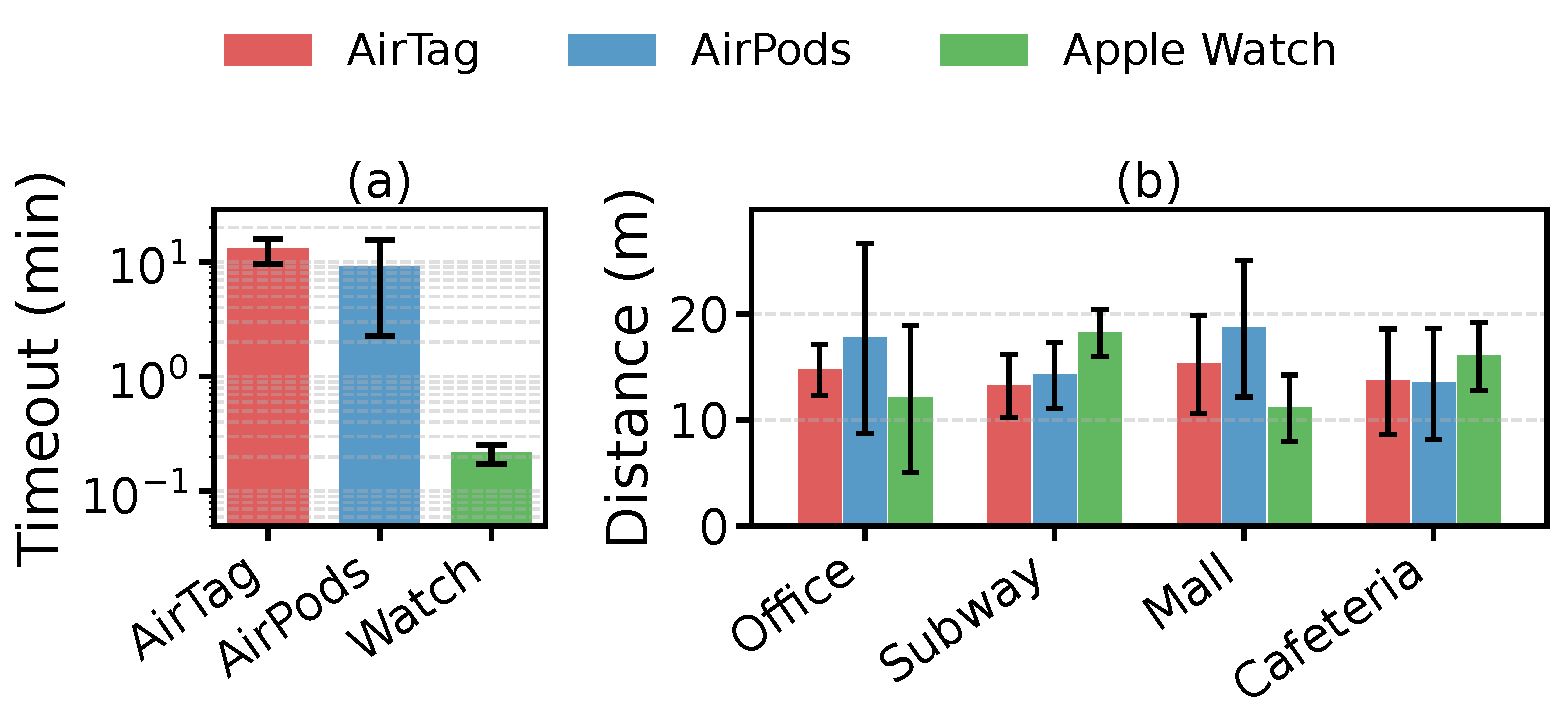
\includegraphics[width=\linewidth]{figs/timeout_disconnect.pdf}
  \caption{E1, lost-state onset (paper Figure 3): per-device time to enter the
  lost state (a, log axis) and the owner-to-device disconnect distance across
  four indoor scenes (b).}
  \Description{Left: a log-scale boxplot of lost-state timeout for AirTag (about 12 minutes), AirPods (variable), and Apple Watch (about 13 seconds). Right: grouped boxplots of disconnect distance, around 10 to 20 metres, across Office, Subway, Mall, and Cafeteria scenes for the three devices.}
  \label{fig:ae_onset}
\end{figure}

\noindent\textbf{(E2) MAC-address rotation period (paper Table~2)} [5~person-min]. The
Find My address-rotation period per device --- Vulnerability~III, which bounds
how long one address can be followed.
\noindent\textbf{Preparation:} \texttt{cd reproduce/2\_mac\_rotation}.\\
\textbf{Execution:} \texttt{python make\_table.py}.\\
\noindent\textbf{Results:} a per-device table (Table~\ref{tab:ae_rotation}) that
reproduces paper Table~2: Apple accessories hold one MAC for $\sim$24\,h, while
iPhone and Apple~Watch rotate every $\sim$15--36\,min.
\texttt{make\_table.py} also writes \texttt{mac\_rotation.pdf} (a log-scale
boxplot of the per-address spread), and \texttt{derive\_durations.py} re-derives
the iPhone column from the shipped capture. The long static window on
accessories is what makes Level-3 tracking practical.

\begin{table}[H]
  \centering
  \caption{E2 output, reproducing paper Table~2: measured Find My MAC-address
  rotation period per device.}
  \label{tab:ae_rotation}
  \begin{tabular}{llc}
    \toprule
    \textbf{Category} & \textbf{Device} & \textbf{MAC rotation period} \\
    \midrule
    Apple Accessories & AirPods Pro & $\sim$24\,h (daily, $\sim$4\,am) \\
                      & AirTag      & $\sim$24\,h (daily, $\sim$4\,am) \\
    \midrule
    Apple Devices     & iPhone      & fixed $\sim$15\,min \\
                      & Apple Watch & 19--36\,min \\
    \bottomrule
  \end{tabular}
\end{table}

\begin{figure*}[t]
  \centering
  \begin{subfigure}[t]{0.310\linewidth}
    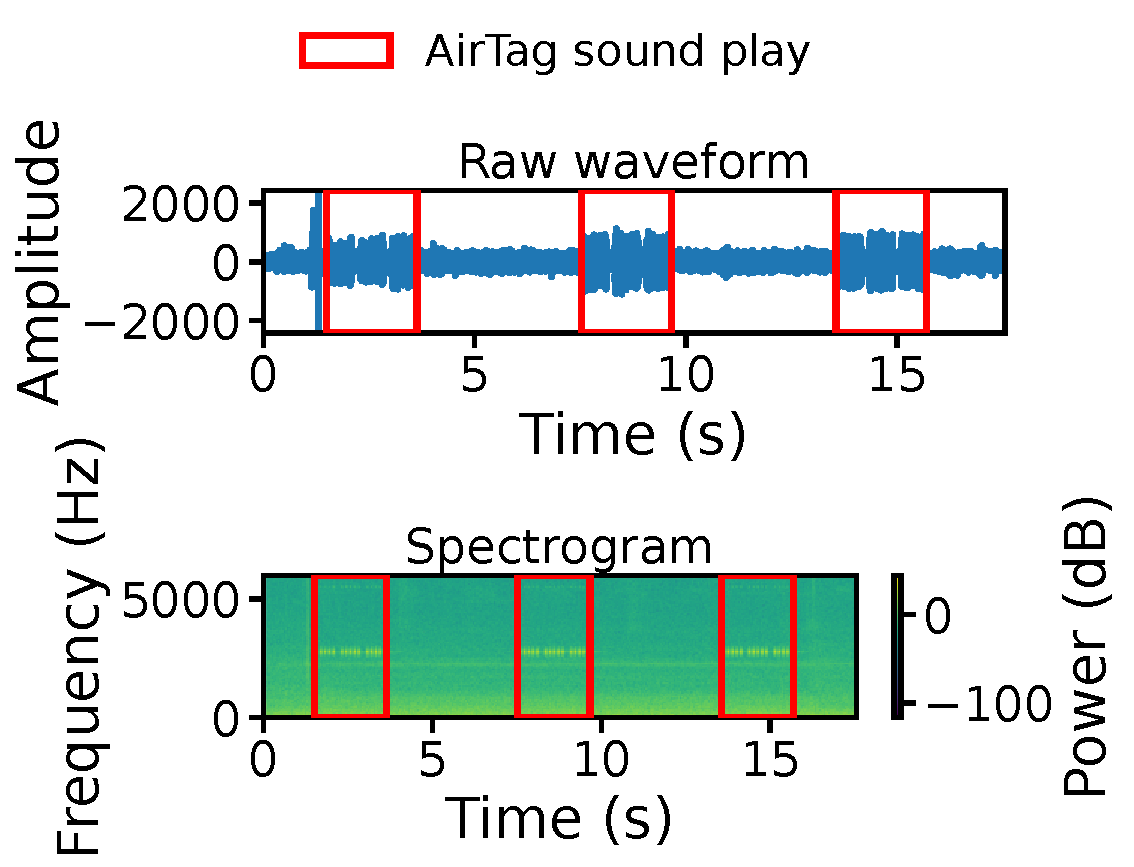
\includegraphics[width=\linewidth]{figs/waveform_spectrogram.pdf}
    \caption{Raw recording (waveform + spectrogram).}
    \label{sf:ae_wave}
  \end{subfigure}\hfill
  \begin{subfigure}[t]{0.377\linewidth}
    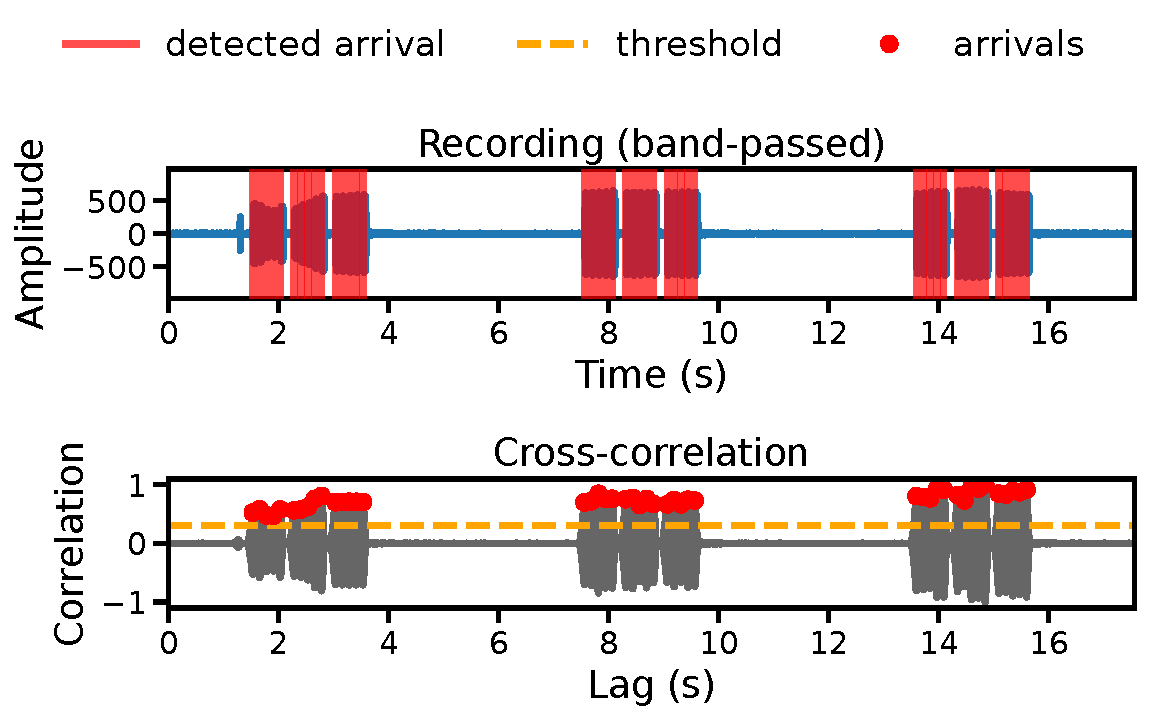
\includegraphics[width=\linewidth]{figs/acoustic_example.pdf}
    \caption{Arrival detection (recording + cross-correlation).}
    \label{sf:ae_acoustic}
  \end{subfigure}\hfill
  \begin{subfigure}[t]{0.274\linewidth}
    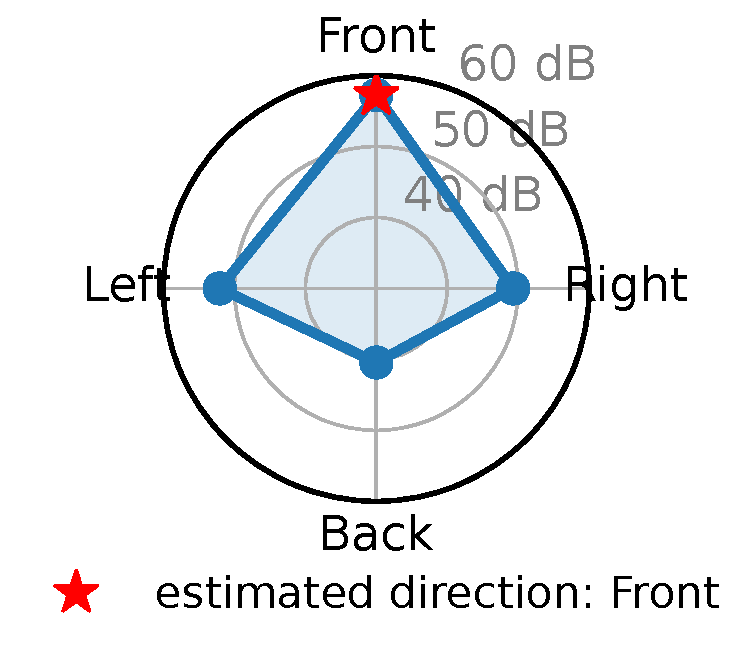
\includegraphics[width=\linewidth]{figs/direction_polar.pdf}
    \caption{Direction-finding result.}
    \label{sf:ae_polar}
  \end{subfigure}
  \caption{E3, acoustic direction finding (Level~1): the top-mic recording (a),
  band-passed and cross-correlated with the chirp template, gives the arrival
  level ($\approx-42.8$\,dB) (b); four body orientations yield the
  direction estimate, here \emph{Front} (c).}
  \label{fig:ae_e1}
\end{figure*}

\noindent\textbf{(E3) Acoustic direction finding (Level~1, paper Figure~6)}
[10~person-min $+$ $<$5~compute-min]. The input is the phone's \emph{top}-mic
channel (\texttt{data/example\_top.pcm}, 16-bit mono PCM at 44.1\,kHz) and the
model chirp template (\texttt{data/template.wav}).
\noindent\textbf{Preparation:} \texttt{cd reproduce/3\_acoustic\_direction}.\\
\textbf{Execution:}
\begin{lstlisting}
python plot_waveform_spectrogram.py  # waveform + spectrogram
python acoustic_example.py           # arrival detection + dB
python plot_direction_polar.py       # direction polar
\end{lstlisting}
\noindent\textbf{Results:} \texttt{plot\_waveform\_spectrogram.py} shows the chirp
energy around 2.6--2.8\,kHz (Figure~\ref{fig:ae_e1}a).
\texttt{acoustic\_example.py} band-passes both signals to that band,
cross-correlates to detect the arrivals, and takes the RMS over each in dB
($\approx-42.8$\,dB; Figure~\ref{fig:ae_e1}b). The four body orientations give
four dB values, which \texttt{plot\_direction\_polar.py} turns into the
contrast-enhanced score $S_k=\alpha A_k+\beta\,(A_k-A_{opp(k)})$
($\alpha{=}0.3,\beta{=}0.7$); the heading $\arg\max_k S_k$ falls at the
\textit{Front} by body shadowing (Figure~\ref{fig:ae_e1}c), reproducing the
paper's Level~1 result.

\noindent\textbf{(E4) RSSI--IMU navigation (Level~2, paper Figure~8)} [10~person-min].
\texttt{SnatchAPP} logs, per BLE reading, the target's RSSI with the phone
heading and the IMU-derived Pedestrian-Dead-Reckoning (PDR) position and step
count (column format in the folder's \texttt{README}); two sample logs are
provided.
\noindent\textbf{Preparation:} \texttt{cd reproduce/4\_rssi\_navigation}.\\
\textbf{Execution:}
\begin{lstlisting}
python plot_trace.py                  # data/nav_trace_1.csv
python plot_trace.py --log data/nav_trace_2.csv
\end{lstlisting}
\noindent\textbf{Results:} the script picks the target device (the
frequently-seen MAC with the highest peak RSSI), reconstructs the walked path
from the logged PDR position, and colours it by RSSI. The path converges on the
target as RSSI rises (e.g.\ $-81\to-39$\,dBm; Figure~\ref{fig:ae_nav}),
reconstructing the paper's Level~2 navigation trace.

\begin{figure}[tbp]
  \centering
  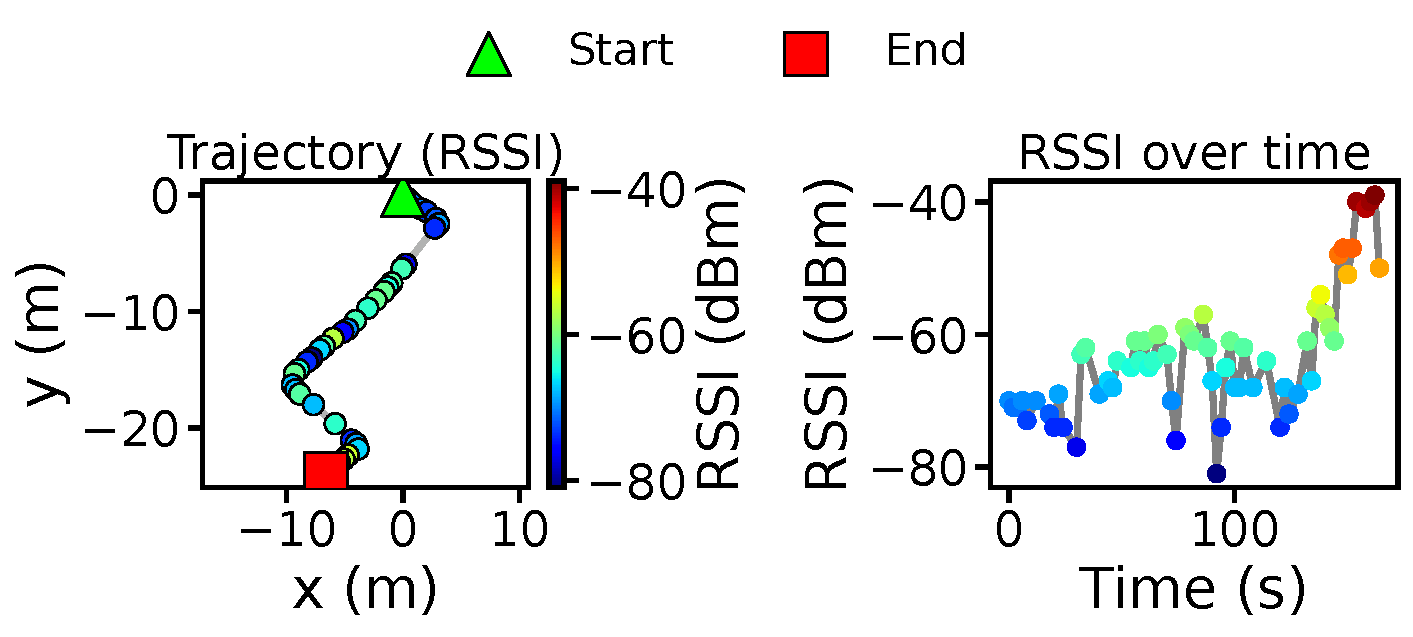
\includegraphics[width=\linewidth]{figs/nav_trace.pdf}
  \caption{E4, navigation trace: the walked PDR trajectory coloured by RSSI
  (left) and RSSI over time (right), converging on the target as RSSI rises.}
  \Description{Left: a 2-D walking trajectory coloured by RSSI, starting at low signal strength and ending at high signal strength near the target. Right: RSSI versus time rising from about -81 to -39 dBm.}
  \label{fig:ae_nav}
\end{figure}

\noindent\textbf{(E5) Spatial--temporal clustering (Level~3, paper Figure~11)} [10~person-min].
Co-located mimicked AirTags (the provided ESP32 firmware) at different distances.
For exact ground truth the script applies the MAC-address rotation in software,
each device rotating independently (the firmware does the same on-device); the
clustering runs blind, on timing and RSSI only.
\noindent\textbf{Preparation:} \texttt{cd reproduce/5\_clustering}.\\
\textbf{Execution:}
\begin{lstlisting}
python cluster.py --log data/clustering_log_3dev.csv  # 3 devices
python cluster.py                                     # 2 devices
\end{lstlisting}
\noindent\textbf{Results:} the script runs the paper's two stages.
\emph{Static profiling} colours the temporal-conflict graph --- a device cannot
advertise two MACs at once, so overlapping MACs seed different clusters --- and
reads off each device's $\sim$30\,s rotation period. \emph{Dynamic stitching}
then attaches each later MAC to the one cluster whose previous MAC has already
ended, breaking ties by RSSI and period. On the three-device log
(Figure~\ref{fig:ae_cluster}), whose RSSI ranges overlap and cross, the temporal
constraint still recovers all three trajectories, defeating MAC rotation as in
the paper's Level~3 result.

\begin{figure}[H]
  \centering
  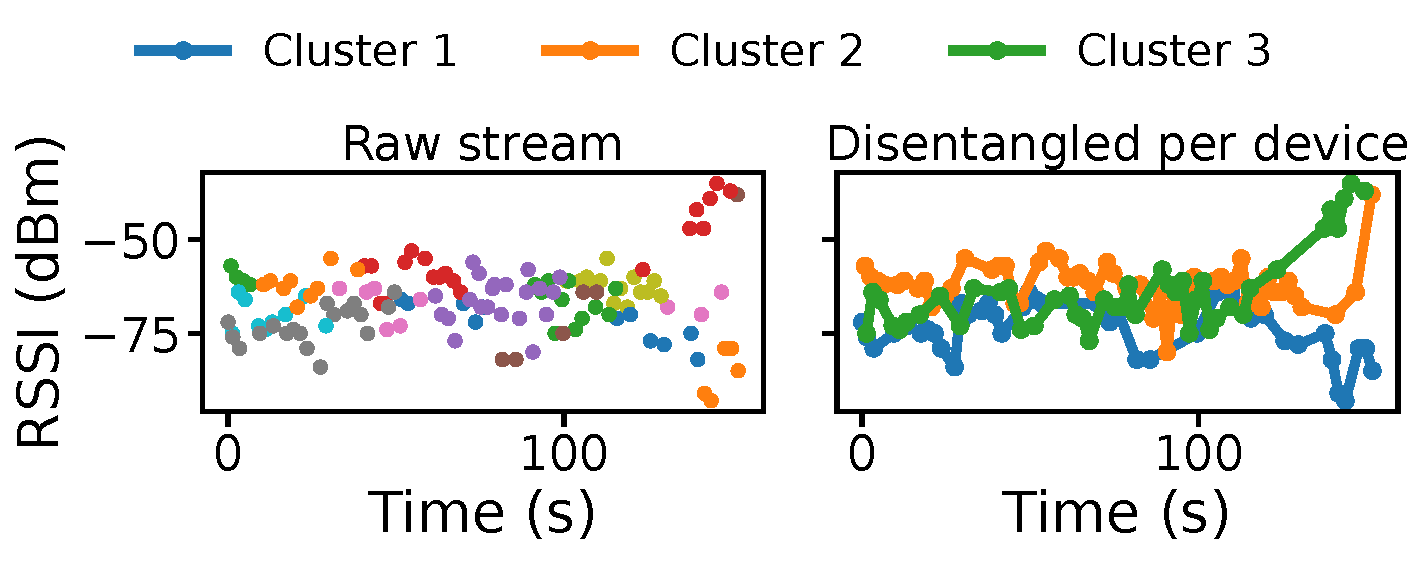
\includegraphics[width=\linewidth]{figs/clustering_trace_3dev.pdf}
  \caption{E5, clustering (three devices): from the fragmented rotated-MAC stream
  (left) the temporal-overlap\,+\,RSSI method recovers the three per-device
  trajectories (right).}
  \Description{Left: RSSI over time for three devices with each rotated MAC a different colour, appearing fragmented. Right: three recovered per-device RSSI trajectories that cross in the middle -- one rising, one falling, one roughly constant.}
  \label{fig:ae_cluster}
\end{figure}

\noindent\textbf{(E6) Maximum attack distance (paper Figures~14--15)} [10~person-min].
Two field sweeps over the attacker-to-device distance (0--80\,m): the BLE
discovery channel and the non-owner sound trigger.
\noindent\textbf{Preparation:} \texttt{cd reproduce/6\_max\_distance}.\\
\textbf{Execution:} \texttt{python plot\_max\_distance.py}.\\
\noindent\textbf{Results:} two dual-axis plots (Figure~\ref{fig:ae_maxdist}):
\emph{(a)}~RSSI decays while the scanned interval rises sharply beyond
$\sim$60\,m (discoverable to tens of metres); \emph{(b)}~the triggered sound is
loud near the device ($\sim$92\,dB), fading to ambient by $\sim$30\,m ---
reproducing Figures~14--15.

\begin{figure}[H]
  \centering
  \begin{subfigure}[b]{0.48\linewidth}
    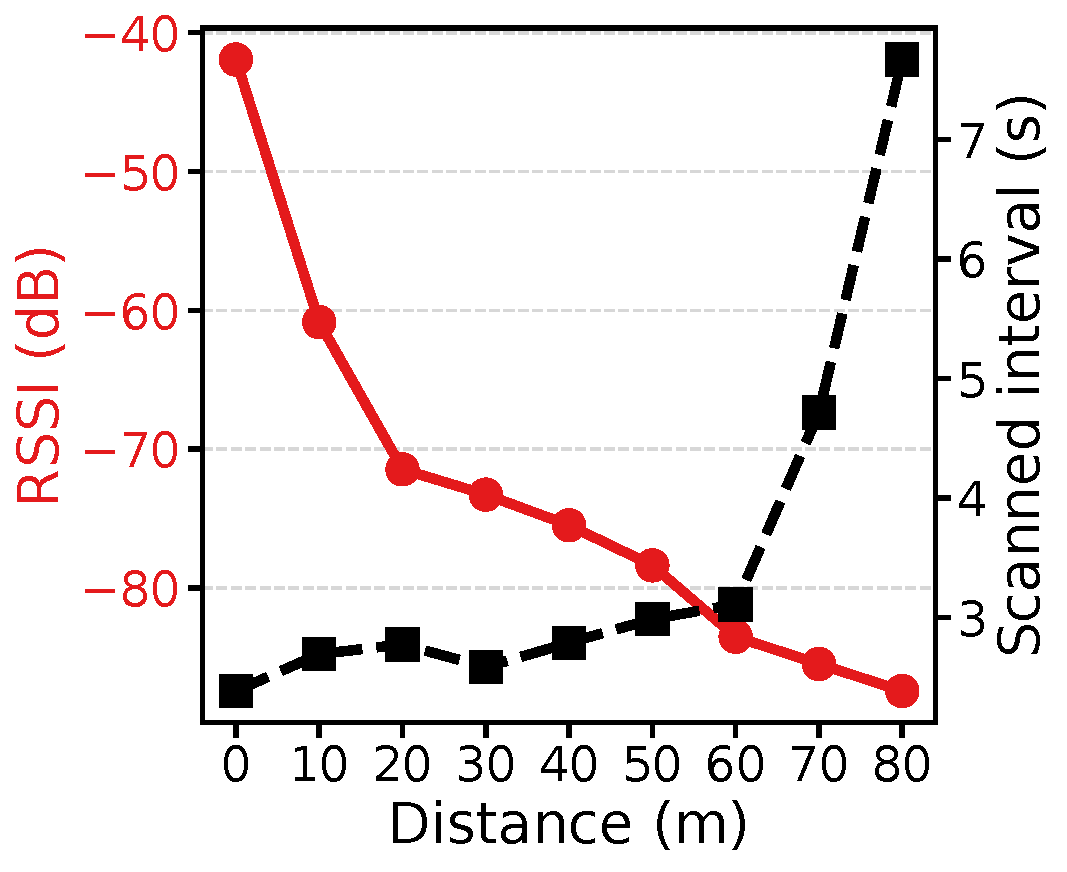
\includegraphics[width=\linewidth]{figs/maxdist_rssi.pdf}
    \caption{BLE discovery range vs distance.}
    \label{sf:maxdist_rssi}
  \end{subfigure}\hfill
  \begin{subfigure}[b]{0.48\linewidth}
    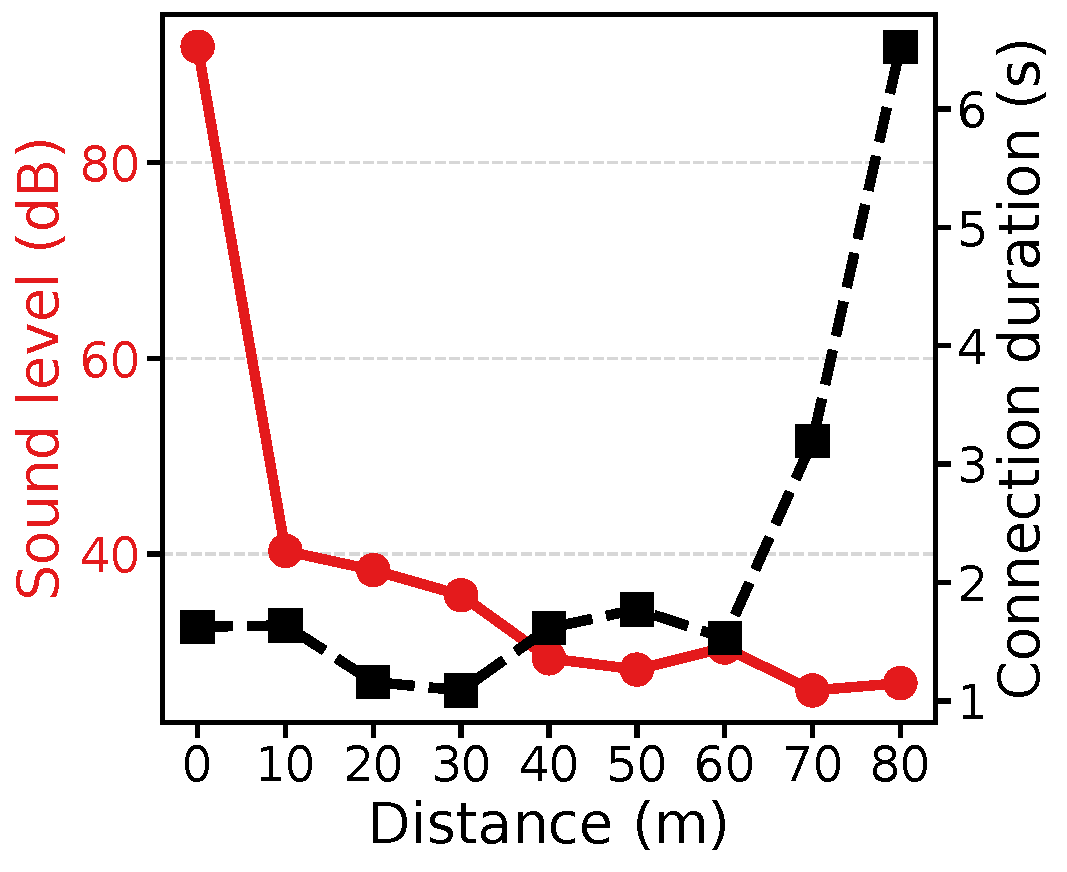
\includegraphics[width=\linewidth]{figs/maxdist_sound.pdf}
    \caption{Sound-trigger range vs distance.}
    \label{sf:maxdist_sound}
  \end{subfigure}
  \caption{E6, maximum attack distance (paper Figures 14--15): the attack's
  BLE-discovery range (a) and non-owner-sound range (b), swept from 0 to 80\,m.}
  \Description{Two dual-axis line plots versus distance from 0 to 80 metres. (a) RSSI decreasing from about -42 to -87 dB while the scanned advertising interval stays near 2.5 s then rises past 60 m. (b) Sound level dropping from about 92 dB at 0 m toward ambient by 30 m, with connection duration rising at the far end.}
  \label{fig:ae_maxdist}
\end{figure}

\noindent\textbf{(E7) End-to-end navigation sample traces (paper Figure~17)} [5~person-min].
Sample walking trajectories from the end-to-end evaluation, one per attack level.
\noindent\textbf{Preparation:} \texttt{cd reproduce/7\_navigation\_traces}.\\
\textbf{Execution:} \texttt{python plot\_traces.py}.\\
\begin{figure}[H]
  \centering
  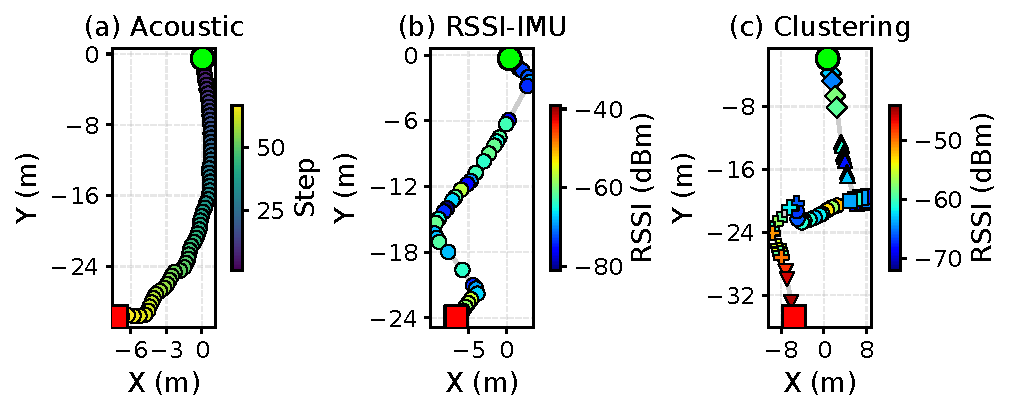
\includegraphics[width=\linewidth]{figs/nav_traces.pdf}
  \caption{E7, sample end-to-end navigation traces (paper Figure~17), one per
  attack level, each homing from green Start to red End on the target.}
  \Description{Three trajectory panels of attacker position in metres. (a) a path coloured by step count. (b) a path with points coloured by RSSI from about -80 to -40 dBm. (c) a path with points coloured by RSSI and many marker shapes for the rotating MAC addresses. Each runs from a green Start marker to a red End marker.}
  \label{fig:ae_traces}
\end{figure}

\noindent\textbf{Results:} three sample trajectories (Figure~\ref{fig:ae_traces}),
one per level: \emph{(a)}~Level-1 acoustic; \emph{(b)}~Level-2 RSSI--IMU
(colour = RSSI); \emph{(c)}~Level-3 under clustering (MAC rotates every
30\,s; colour = RSSI, shape = MAC). Each converges on the target
(green Start $\to$ red End); panel~(b) reuses the (E4) trace.

\end{document}
